\chapter{Metodologia}


\resumodocapitulo{Neste capítulo explicaremos com mais detalhes a arquitetura do trabalho \cite{FullResolution2017Toderici}, o método para elaboração da  de treinamento,  uma função de custo para promover esparsidade no código binário. Além disso, abordamos um método simples para alocação de bits com base em um alvo de qualidade}.  

\section{Arquitetura} \label{sec:arq}

Nessa seção explicaremos o método para treinamento do modelo ao longo das iterações, os formatos dos tensores nas saídas de cada camada da rede, e como se dá a formação do código binário de uma imagem.   

Usamos o autocodificador com camadas LSTM-convolucional proposto por \cite{FullResolution2017Toderici} e apresentado na Figura \ref{fig:toderici3}. 
Decidimos que a rede irá receber a informação residual do estágio anterior, dada por $ r_t = r_{t-1}$ - $r'_{t-1}$, e será treinada para reconstruí-la. Dessa forma, a reconstrução de uma imagem $x$ será progressivamente. Essas duas características estão resumidas na próxima Equação:

\begin{equation}
\label{eq:model_1it}
\begin{aligned}
r_{0} &=x\\
x'_0  &=0 \\
b_{t} &= B(E_{t}(r_{t-1})) \\
r'_{t-1} &= D_{t}(b_{t}) \\
r_{t} &= r_{t-1}- r'_{t-1} \\
x'_t &= r'_{t-1} + x'_{t-1}  
\end{aligned}
\end{equation}

Originalmente, esse método foi apresentado em \cite{Variable2016Toderici} para treinar autocodificadores de camadas não-recorrente. 
Ele difere um pouco do apresentado em \cite{FullResolution2017Toderici} e descrito pela Equação \ref{eq:ae_full},  pois nele os autores usam o valor de $x-x'_{t-1}$ como  informação residual de entrada no estágio $t$, ou seja, o resíduo em relação à imagem original.
A Figura \ref{fig:rede_toderici} mostra a rede ``desenrolada'' no tempo. Para simplificar a representação, omitimos as camadas \acrshort{pe}. 

\begin{figure}
	\centering
	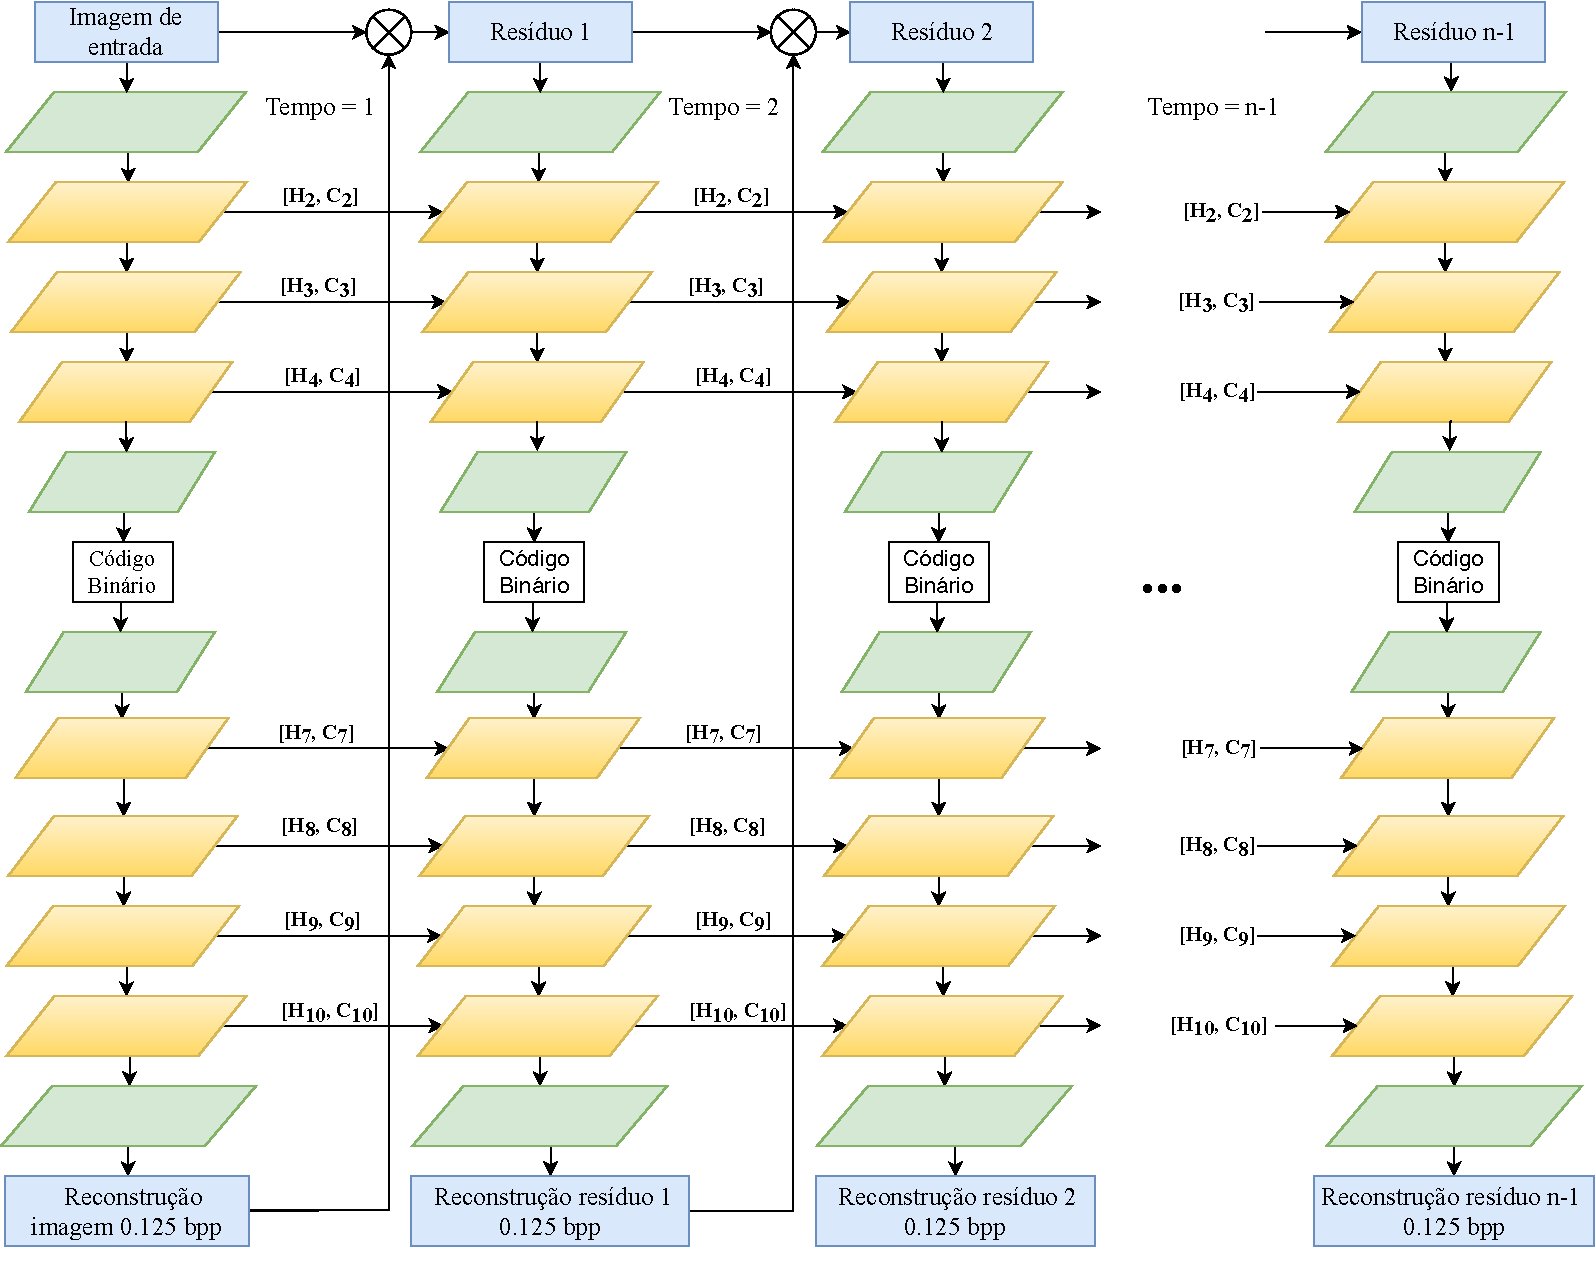
\includegraphics[width=0.90\textwidth]{figuras/redeTCC.pdf}
	\caption[Autocodificador desenrolado no tempo]{Representação do autocodificador ao decorrer de $n$ estágios. Os losangos verdes e laranjas representam as camadas Conv2d e \acrshort{conv2dlstm}, respectivamente.  Na primeira iteração os valores de $C_t$ e  $H_t$ em cada \acrshort{conv2dlstm} são zeros.  As setas horizontais evidenciam o $loop$ dessas camadas. Em cada interação o autocodificador recebe o resíduo da reconstrução anterior como entrada e tenta reconstrói-lo ao final da iteração usando 0,125 bits por pixel. }
	\label{fig:rede_toderici}
\end{figure}

Usamos as camadas \acrshort{conv2dlstm} descritas pela Equação \ref{eq:conlstm} para capturar as dependências espaciais dos resíduos que formam uma sequência. A Figura \ref{fig:convlstm} detalha essa camada com $k$ mapas de recursos. 

\begin{figure}[ht]
	\centering
	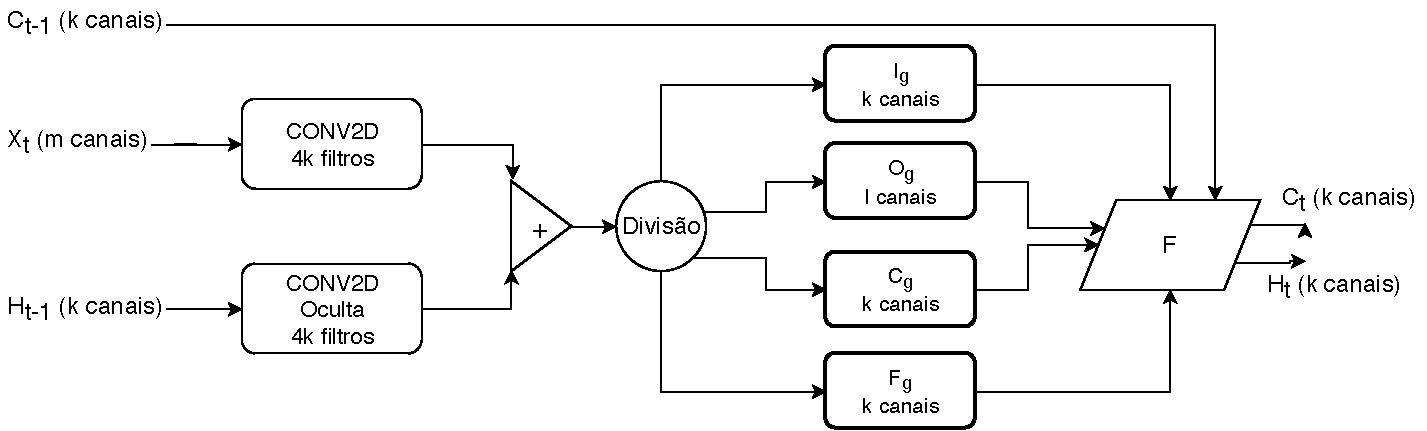
\includegraphics[width=0.90\textwidth]{figuras/convlstm.pdf}
	\caption[Conv2DLSTM]{Camada convolucional recorrente com $k$ filtros. Sendo $X_t$ o elemento atual da nossa sequência, com $m$ canais. Os tensores $H_{t-1}$ e $C_{t-1}$ representam a saída e o estado de célula gerados por essa unidade na etapa anterior. As saídas de ambas as convoluções têm o mesmo número de canais, $4\times k$, para serem somadas ponto-a-ponto. Em seguida, o novo tensor é separado em 4 novos tensores de $k$ canais. Eles representarão as portas de entrada, esquecimento, célula e saída. A função $F$ irá operar nas portas e no tensor $C_{t-1}$ para fornecer $C_t e H_t$, segundo as equações em \ref{eq:conlstm}.}
	\label{fig:convlstm}
\end{figure}

Por construção, a arquitetura da rede determina que a saída do codificador é um conjunto de bits da forma $\frac{H}{16} \times \frac{W}{16} \times 32$ (por cada iteração). Os valores de $H$ e $W$ são, respectivamente, a altura e largura da imagem de entrada. Isso nos fornece $\frac{H \times W}{8}$ bits e podemos calcular a taxa nominal por iteração $R_{it}$, em bits por pixel:

\begin{equation}
\label{eq:bpp}
R_{it} = \frac{\frac{H \times W}{8}}{H \times W} =  \frac{1}{8}\text{ bpp} 
\end{equation}

Então, obtemos a taxa nominal $R$ na iteração $k>0$ como $R =\frac{k}{8} $.  Dessa forma, podemos controlar a quantidade de bits por pixel que enviamos ao decodificador com o passo de $1/8$. Aplicando a Equação \ref{eq:compressao} obtemos a taxa compressão nominal $C$ na iteração $k$: 

\begin{equation}
\label{eq:tc}
C = \frac{24 \times H \times W}{k \times \frac{H \times W}{8}} =  \frac{192}{k} 
\end{equation}


Os detalhes do autocodificador podem ser consultados na Tabela \ref{table:aerc} para uma entrada com formato $32 \times 32 \times 3$. O tamanho do lote está omitido dessa representação, contudo,  ele ocupa mais uma dimensão, e possui valor fixo (pode ser diferente no último lote de uma imagem) durante todas as operações realizadas pela rede.
\begin{table}[htbp]
	\caption{Parâmetros das operações no autocodificador.}
	\begin{adjustbox}{width=\columnwidth,center}
		\begin{tabular}{|c|c|c|c|c|c|c|}
			\hline
			\rowcolor[HTML]{EFEFEF} 
			\textbf{Camada} & \textbf{\begin{tabular}[c]{@{}c@{}}Formato de\\  saída\end{tabular}} & \textbf{\begin{tabular}[c]{@{}c@{}}Núcleo \\ Convolucioal\\ Normal/Oculto\end{tabular}} & \textbf{Passo} & \textbf{Preenchimento} & \textbf{\begin{tabular}[c]{@{}c@{}}Função de\\ Ativação\end{tabular}} & \textbf{\begin{tabular}[c]{@{}c@{}}Número de\\ Parâmetros\end{tabular}} \\ \hline
			Conv2D          & 16x16x64                                                             & 3x3/-                                                                                   & 2              & 1                  & Identididade                                                          & 1728                                                                    \\ \hline
			Conv2DLSTM      & 8x8x256                                                              & 3x3/1x1                                                                                 & 2              & 1                  & Logística                                                               & 851968                                                                  \\ \hline
			Conv2DLSTM      & 4x4x512                                                              & 3x3/1x1                                                                                 & 2              & 1                  & Logística                                                               & 5767168                                                                 \\ \hline
			Conv2DLSTM      & 2x2x512                                                              & 3x3/1x1                                                                                 & 2              & 1                  & Logística                                                               & 10485760                                                                \\ \hline
			Conv2D          & 2x2x32                                                               & 1x1/-                                                                                   & 1              & 0                 & Tanh                                                                  & 16384                                                                   \\ \hline
			Binarizador     & 2x2x32                                                               & -                                                                                       &                &                        &                                                                       &                                                                         \\ \hline
			Conv2D          & 2x2x512                                                              & 1x1/-                                                                                   & 1              & 1                  & Identididade                                                          & 16384                                                                   \\ \hline
			Conv2DLSTM      & 2x2x512                                                              & 3x3/1x1                                                                                 & 1              & 1                  & Logística                                                               & 10485760                                                                \\ \hline
			PE             & 4x4x128                                                              & -                                                                                       &                &                        &                                                                       &                                                                         \\ \hline
			Conv2DLSTM      & 4x4x512                                                              & 3x3/1x1                                                                                 & 1              & 1                  & Logística                                                               & 3407872                                                                 \\ \hline
			PE             & 8x8x128                                                              & -                                                                                       &                &                        &                                                                       &                                                                         \\ \hline
			Conv2DLSTM      & 8x8x256                                                              & 3x3/1x1                                                                                 & 2              & 1                  & Logística                                                               & 1441792                                                                 \\ \hline
			PE             & 16x16x64                                                             & -                                                                                       &                &                        &                                                                       &                                                                         \\ \hline
			Conv2DLSTM      & 16x16x128                                                            & 3x3/1x1                                                                                 & 2              & 1                  & Logística                                                               & 360448                                                                  \\ \hline
			PE             & 32x32x32                                                             & -                                                                                       &                &                        &                                                                       &                                                                         \\ \hline
			Conv2D          & 32x32x3                                                              & 1x1/-                                                                                   & 1              & 1                  & Tanh                                                                  & 96                                                                      \\ \hline
			\multicolumn{6}{|c|}{Total de parâmetros}                                                                                                                                                                                                                                                          & 32835360                                                                \\ \hline
		\end{tabular}\quad
	\end{adjustbox}
	\label{table:aerc}
\end{table}
\subsection{Binarização}

O processo de binarização adotado foi o descrito na seção \ref{subsec:bin} e proposto em \cite{Variable2016Toderici}.
Na prática, para tornar esse processo estocástico,  definimos um valor $u$ entre 0 e 1 obtido de uma distribuição uniforme,  $u \in \mathcal{U}[0,1]$ e podemos reescrever a Equação \ref{eq:quant2}  para obter o erro $\epsilon$ da quantização:

\begin{equation}
\label{eq:quant}
\begin{aligned}
\epsilon \ = \left\{
\begin{array}{ll}
1 - x, \text{ se $u$}  \leq \frac{1 + x}{2} \\
-x - 1, \text{ se $u$} > \frac{1 + x}{2}
\end{array}
\right. \\
\end{aligned}
\end{equation}
A binarização será feita com valores -1 e 1, e usamos o truque apresentado em \ref{subsec:bin} para conseguir treinar o modelo com essa camada não diferenciável. 

%\section{Taxas de compressão}



%A Figura \ref{fig:modelo} mostra a arquitetura de uma única iteração do nosso modelo.  Nela temos 4 camadas no encoder: 3 convolucionais e 1 RNN-Conv; 1 camada de binarização do tipo convolucional; e 6 camadas no enconder: 2 convolucionais e 4 unidades RNN-Conv.  As camadas convolucionais são utilizadas especialmente para extrair os recursos das imagens essenciais para garantir a reconstrução de imagens com a menor perda possível. Já as camadas recorrentes do tipo LSTM são empregadas para capturar as dependências entre os patches de entrada e os resíduos gerados nas iterações.   

%\begin{figure}[h]
%	\centering
%	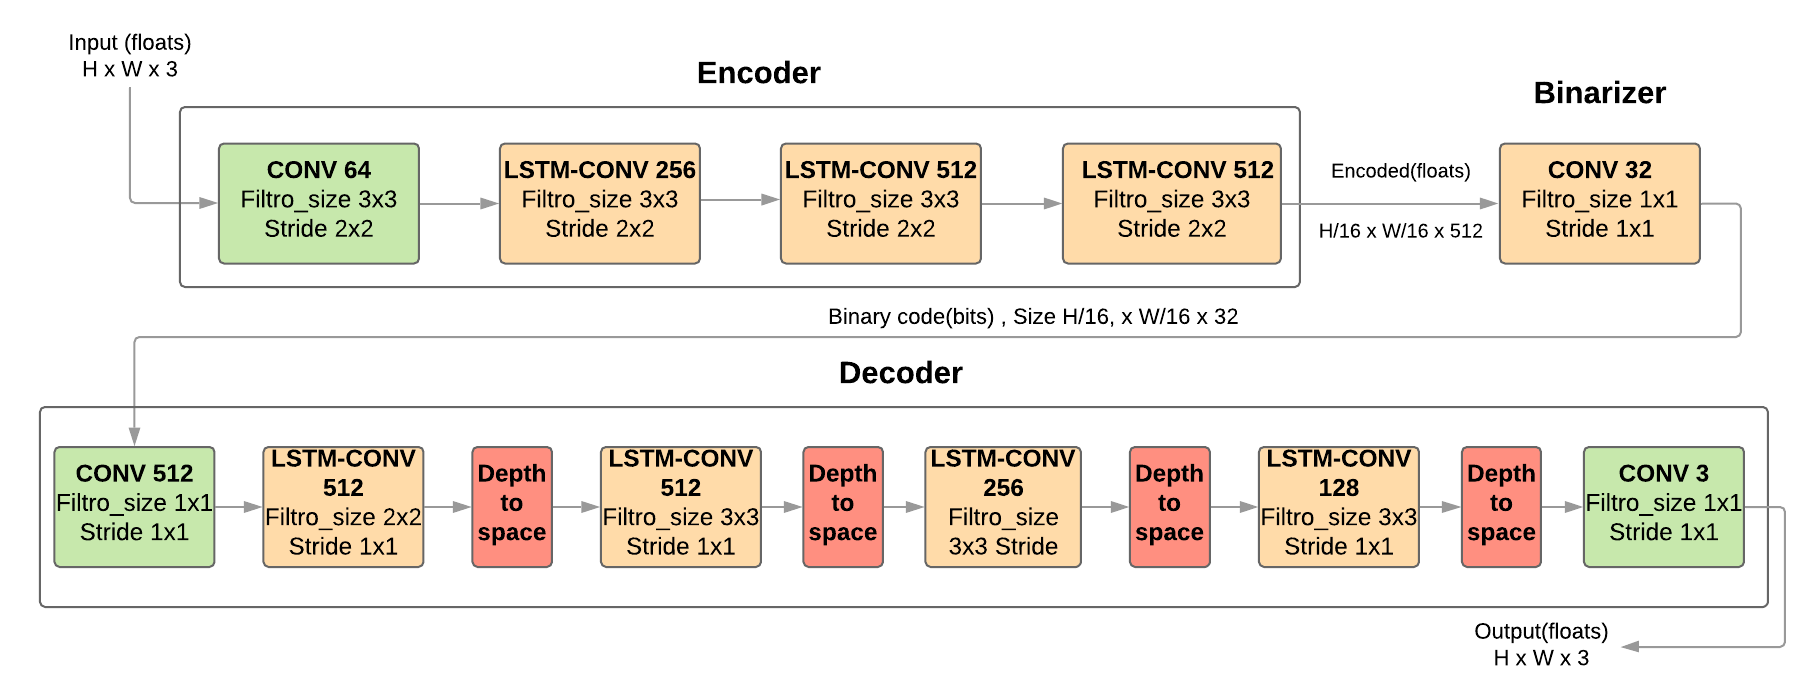
\includegraphics[width=0.90\textwidth]{figuras/arquitetura_rede.png}
%	\caption{Representação de uma iteração do autoencoder \cite{Variable2016Toderici}.}
%	\label{fig:modelo}
%\end{figure}




%Nas unidades RNN-Conv ilustradas na figura \ref{fig:modelo} o tamanho do filtro e o stride refere-se a primeira convolução, a segunda convolução sempre terá filtros de dimensão 1x1 com stride 1x1; e o número de filtros refere-se ao número de canais da LSTM e 1/4 do número de canais das camadas convolucionais dessa unidade.



\subsection{Formato do fluxo de bits}

A arquitetura será otimizada para reconstruir blocos de $32 \times 32$ pixels, uma vez que os modelos serão treinados com imagens dessa dimensão. Portanto, durante os testes, devemos dividir as imagens em blocos $32 \times 32$ pixels. 

Considerando que o número de blocos gerados é igual a $n$ e desejamos agrupá-los em lotes de tamanho $l$ e reconstruídos passando $k$ vezes pela rede, então teremos:
\begin{enumerate}
	\item Na primeira iteração, o modelo irá tomar os primeiros $l$ blocos da imagem na ordem direita para esquerda e de cima para baixo. 	\item Eles são codificados pela rede do codificador para gerar o código binário parcial de formato $l \times 2 \times 2 \times 32$ conforme a tabela \ref{table:aerc};
	\item Em seguida, decodificamos esse lote e computamos o resíduo;
	\item  Esse resíduo é codificado para gerar um novo código binário $l \times 2 \times 2 \times 32$ que é concatenado com o anterior para formar $2 \times l \times 2 \times 2 \times 32$;
	\item Esse processo se repete até concluirmos as $k$ iterações na rede, e ao final da codificação de um lote o nosso código binário é da forma $k \times l \times 2 \times 2 \times 32$. 
\end{enumerate}

O número de vezes que devemos realizar o processo descrito acima para codificar a imagem inteira é igual a $\frac{n}{l}$. Portanto, o código binário final é da forma $\frac{n}{l} \times k \times l \times 2 \times 2 \times 32$. Obviamente, o número de bits deste código independe do tamanho de lote escolhido. 


\section {Base de Dados}

Nesta seção explicamos o processo de construção das bases de dados de treinamento seguindo um método utilizado em \cite{DeliverableJuly}.

%Essa é uma das principais escolhas para treinar qualquer algoritmo de redes neurais.  

Idealmente, desejamos obter uma base de dados de treinamento a fim de tornar o modelo capaz de comprimir satisfatoriamente (desempenho semelhante ao JPEG2000) imagens naturais com diferentes características de tamanho, componentes de frequência, entropia etc. 

Primeiro, selecionamos imagens de bases de dados distintas que não passaram por nenhum processo de compressão com perdas. Assim, preservamos as componentes de frequência das imagens naturais. Essas imagens foram obtidas dos seguintes conjuntos de dados:

\begin{enumerate}
	\item Conjunto de dados CLIC \cite{bib:clic} (\textit{Challenge on Learned Image Compression}) - Imagens de alta qualidade.
	\subitem \textit{Professional} - validação: 41 imagens
	\subitem \textit{Professional} - treinamento: 585 imagens;
	\subitem \textit{Mobile} - validação: 61 imagens;
	\subitem \textit{Mobile} - treinamento: 1048 imagens.
	\item Conjunto de dados DIV2K \cite{bib:div2k} (\textit{DIVerse 2K resolution high.
		quality image}) - Imagens de alta resolução
	\subitem Treinamento: 800 imagens;
	\subitem Validação: 100 imagens.
	\item Conjunto de dados Ultra-Eye \cite{bib:ultraeye} (\textit{Ultra-Eye: UHD and HD images eye tracking datase}) - Alta qualidade e alta resolução.
	\subitem HD: 38 imagens;
	\subitem UHD: 40 imagens.
\end{enumerate}

%O bloco que apresentou maior entropia foi definido como uma referência de 100\% de entropia. 

Em seguida, recortamos as imagens em blocos de tamanho $32 \times 32$ e salvamos em formato PNG. Esse procedimento gerou 6.231.440 blocos. Apresentamos na Figura \ref{fig:histdatabase} um histograma do tamanho desses blocos. Essa medida é usada aqui como uma estimativa da entropia do bloco. Então, separamos os blocos em 5 base de dados observando os seguintes critérios:


\begin {enumerate}
\label{list:bds}
\item Banco de dados 0 (BD0). Todos os blocos cuja entropia seja inferior aos 20\% dos blocos de mais baixa entropia . Total: 1.248.978 blocos. 
\item Banco de dados 1 (DB1). Todos os blocos no intervalo de 40\% a 60\% de entropia. Total: 1.251.421 blocos.
\item Banco de Dados 2 (DB2). Todos os blocos correspondentes aos 20\% de mais alta entropia. Total: 1.248.725 blocos.
\item Banco de Dados 3 (DB3). Sorteio de 20\% dos blocos que compõem toda a base de dados. Total: 1.247.033 blocos
\item Banco de Dados 4 (DB4). Sorteio de 20\% dos blocos cuja entropia pertença aos 50\% de maior entropia. Total: 1.246.698 blocos
\end{enumerate}


%\begin {enumerate}
%\label{list:bds}
%\item Banco de dados 0 (BD0). Todos os blocos cuja entropia seja menor que 20\% do valor da entropia de %referência. Total: 1.248.978 blocos. 
%\item Banco de dados 1 (DB1). Todos os blocos no intervalo de 40\% a 60\% de entropia de referência. %Total: 1.251.421 blocos.
%\item Banco de Dados 2 (DB2). Todos os blocos correspondentes com pelo menos 80\% da entropia de %referência. Total: 1.248.725 blocos.
%\item Banco de Dados 3 (DB3). Sorteio de 20\% dos blocos que compõem toda a base de dados. Total: %1.247.033 blocos
%\item Banco de Dados 4 (DB4). Sorteio de 20\% dos blocos cuja entropia varia de 50\% a 100\%. Total: %1.246.698 blocos
%\item Banco de Dados 5 (DB5). Todos os blocos cuja entropia varia de 50\% a 100\%ossa referência. Total: %2.287.520 blocos
%\end{enumerate}


\begin{figure}[htbp]
\centering
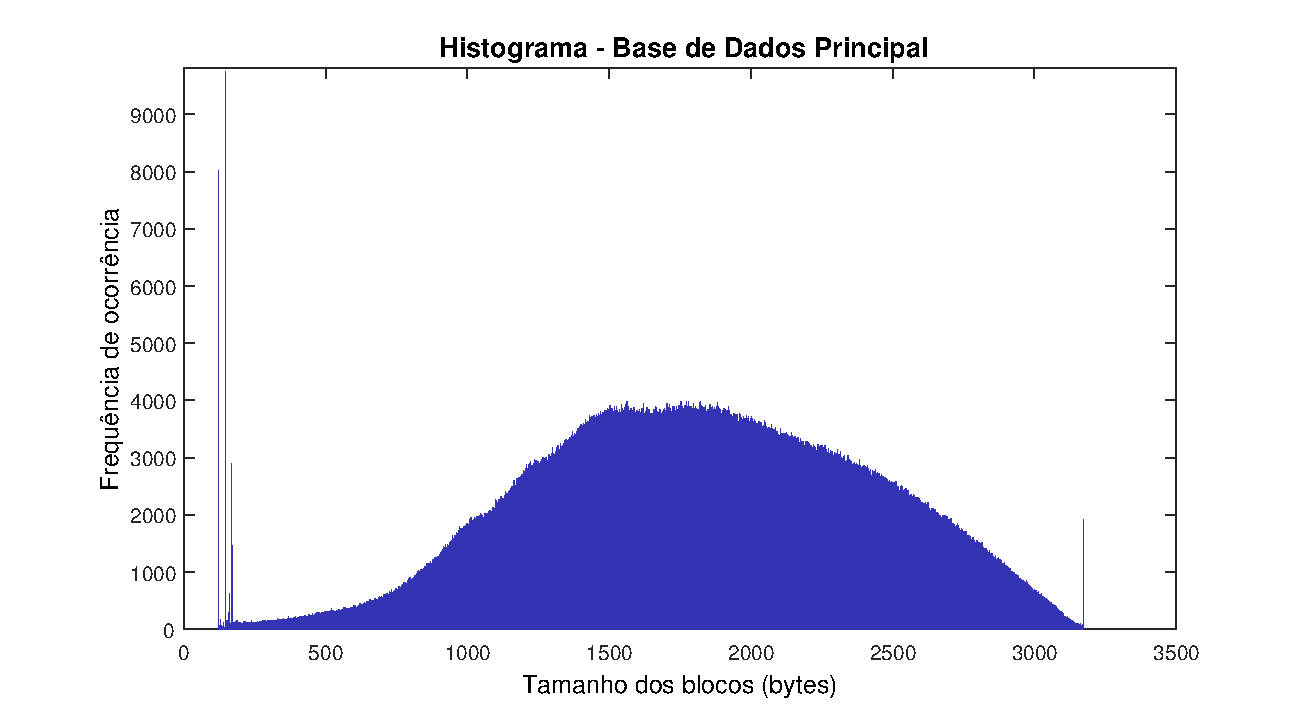
\includegraphics[width=0.80\textwidth]{figuras/hist.eps}
\caption[Histograma de todo o banco de dados]{Histograma de todo o banco de dados}
\label{fig:histdatabase}
\end{figure}

%Por construção, não há sobreposição entre os bancos de dados 0, 1 e 2. No entanto, existem sobreposições de informações entre os bancos de dados 3 e 4. 

Os histogramas dessas bases, exceto a 5, estão ilustrados nas Figuras \ref{fig:database0}, \ref{fig:database1}, \ref{fig:database2}, \ref{fig:database3} e \ref{fig:database4}.

\begin{figure}
\centering
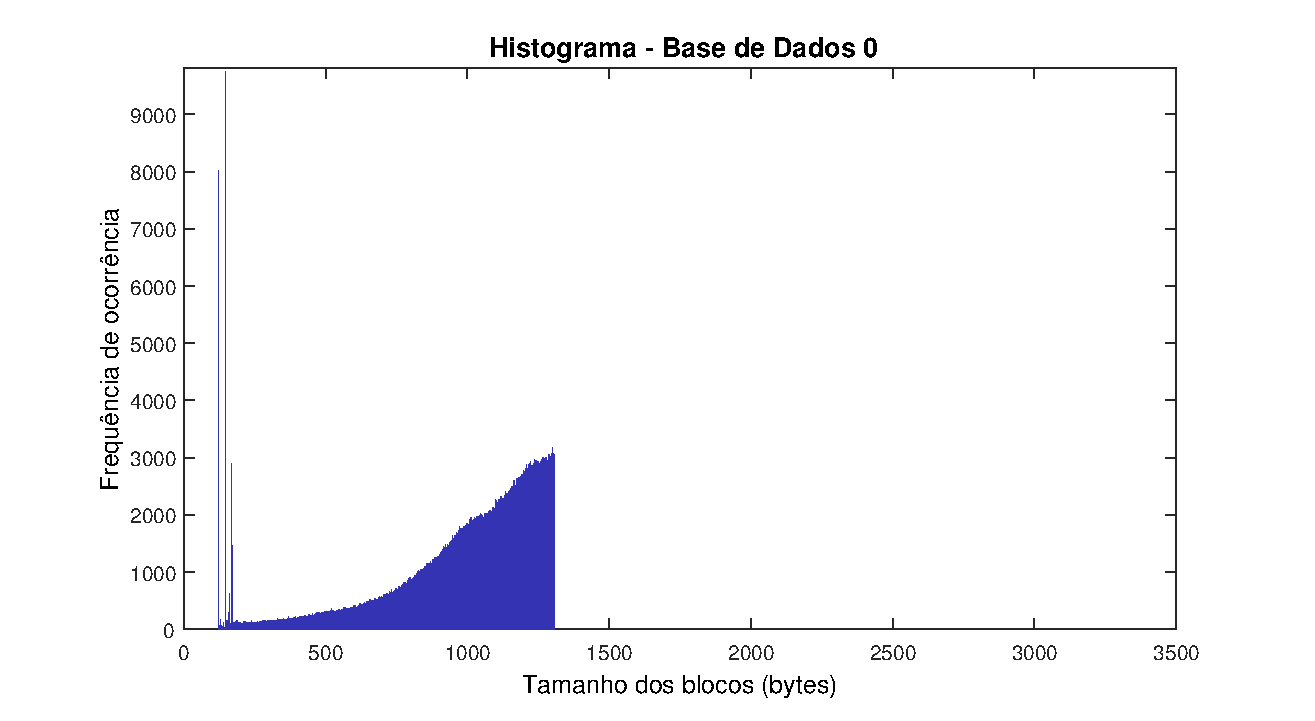
\includegraphics[width=0.8\textwidth]{figuras/hist0.eps}
\caption[Histograma de  baixa entropia -  DB0.]{Histograma de  baixa entropia -  DB0.}
\label{fig:database0}
\end{figure}

\begin{figure}
\centering
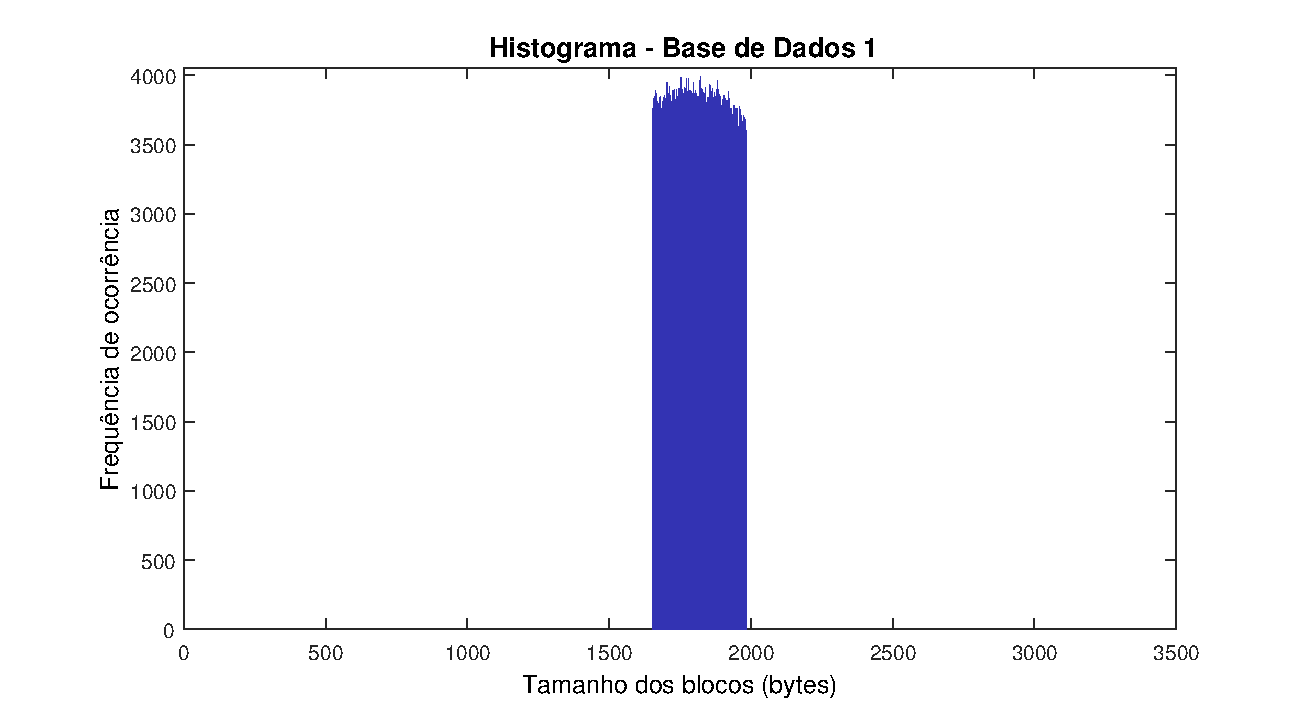
\includegraphics[width=0.80\textwidth]{figuras/hist1.eps}
\caption[Histograma de entropia média - DB1.]{Histograma de entropia média - DB1.}
\label{fig:database1}
\end{figure}

\begin{figure}
\centering
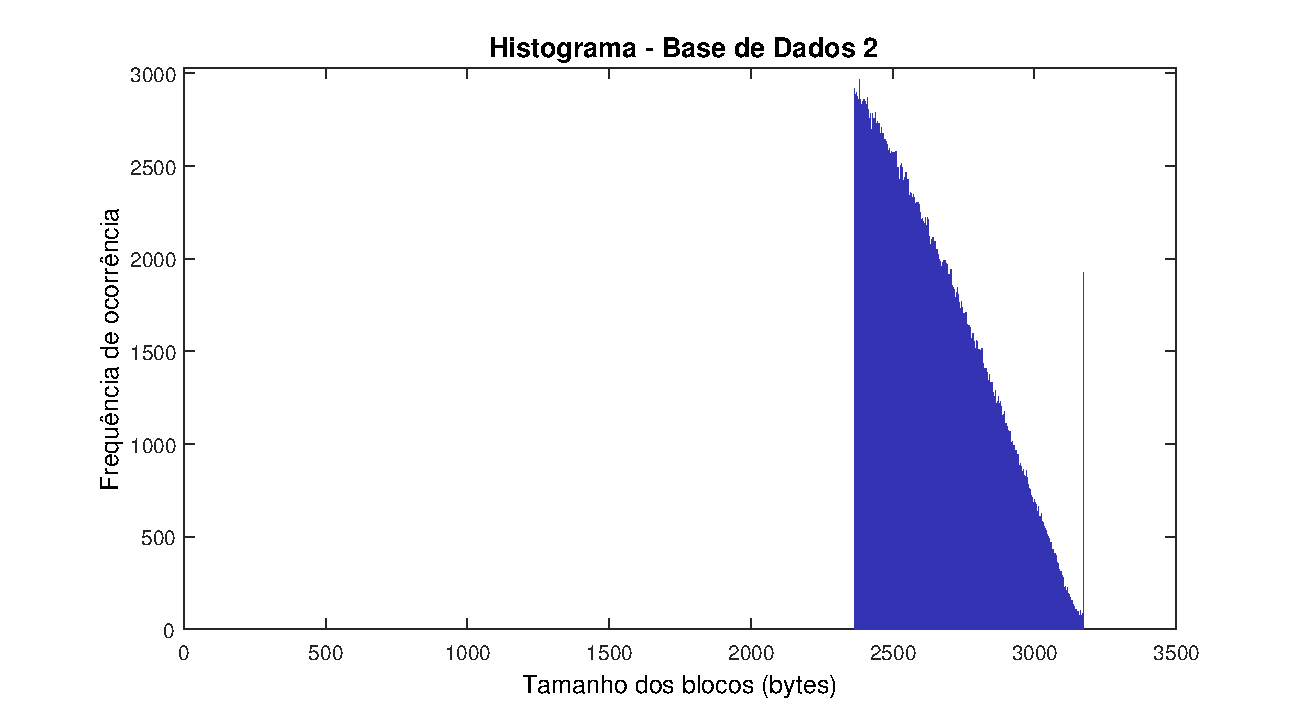
\includegraphics[width=0.8\textwidth]{figuras/hist2.eps}
\caption[Histograma de entropia alta - DB2.]{ Histograma de entropia alta - DB2.}
\label{fig:database2}
\end{figure}

\begin{figure}
\centering
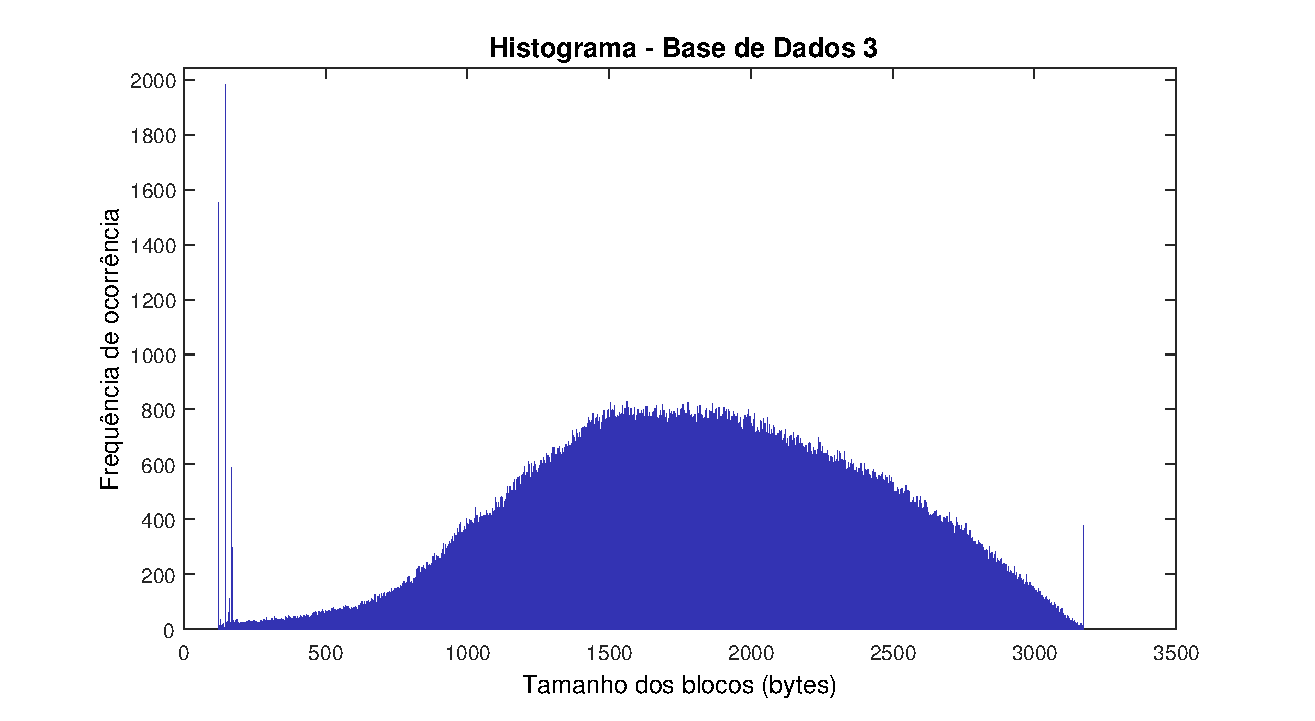
\includegraphics[width=0.80\textwidth]{figuras/hist3.eps}
\caption[Histograma da entropia aleatória - DB3.]{Histograma de entropia aleatória - DB3.}
\label{fig:database3}
\end{figure}

\begin{figure}
\centering
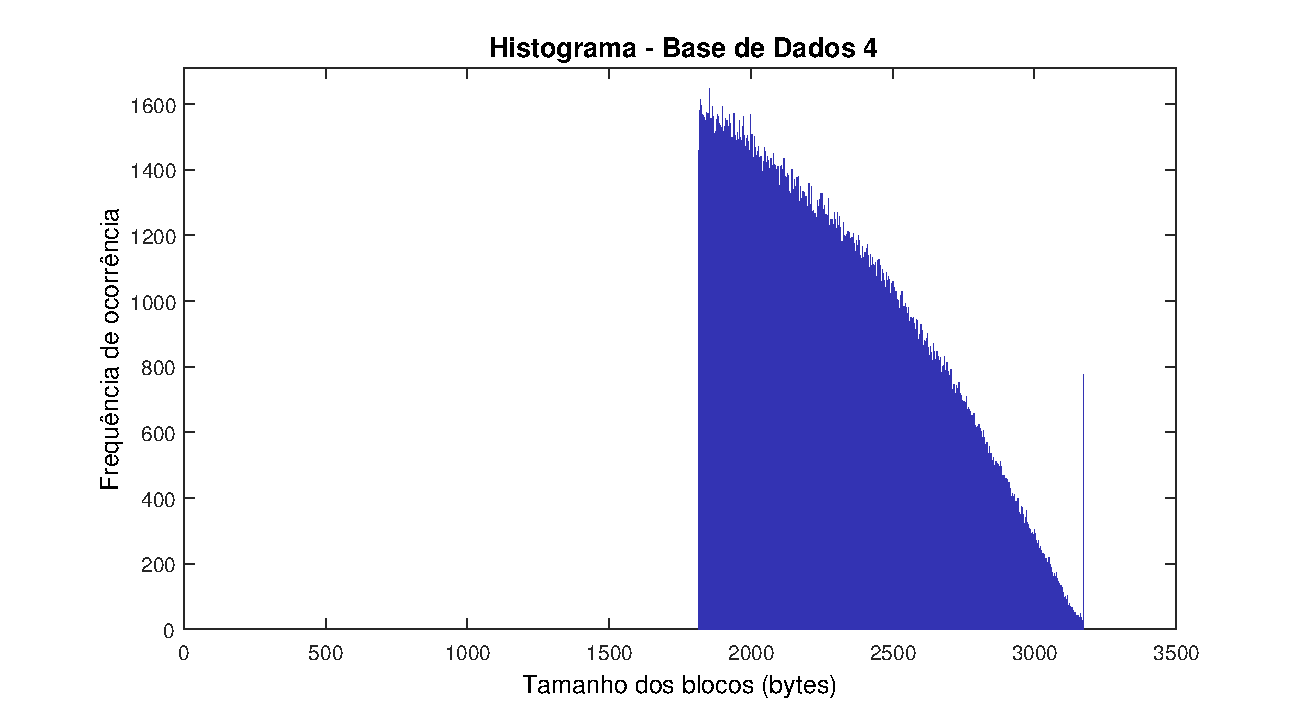
\includegraphics[width=0.8\textwidth]{figuras/hist4.eps}
\caption[Histograma de entropia alta - DB4.]{Histograma de entropia alta - DB4..}
\label{fig:database4}
\end{figure}

Os testes consistiram em treinar a rede usando cada uma das bases e com os mesmos hiperparâmetros. Os modelos gerados são comparados entre si usando as métricas de qualidade.Veremos que a DB4 obteve o melhor resultado, e justificou a elaboração de uma nova base de dados obedecendo a regra.

\begin {enumerate}
\item Banco de Dados 5 (DB5). Todos os blocos cuja entropia varia de 50\% a 100\% em relação ao bloco com maior entropia. Total: 2.287.520 blocos
\end{enumerate}

A base de dados da Kodak \cite{kodak} formada por 24 imagens naturais foi empregada em todos os testes realizados neste trabalho.  

\section {Função de Custo}
Nessa seção, discutimos o procedimento para a escolha da função de custo (ou de perdas) da arquitetura. Em princípio, consideramos apenas a distorção, em segundo momento adicionamos uma regularização na tentativa de controla a entropia do código latente gerado.

\subsection{Otimização por distorção}

%Na hipótese de haver tal função, poderíamos definir uma função de erro em relação à métrica ideal como função de custo e minimizar o seu valor ao longo do aprendizado do modelo. 

A função de custo é uma escolha importante nos treinamentos de \acrshort{rna}. No problema de compressão de imagens a escolha dessa função tem o agravante de não haver consenso entre os pesquisadores de uma métrica ideal para avaliar a qualidade entre uma imagem original e a sua versão reconstruída como relatado em \cite{Priming2017Johnston,End2016Balle}.   
Em nossa análise, usamos as funções conhecidas para medir distorção entre uma imagem e sua reconstrução, tais como \acrshort{mse}, \acrshort{mae}, e uma versão diferenciável de 1-\acrshort{ssim}. Em dois testes, modificamos o espaço de cores dos blocos de \acrshort{rgb} para \acrshort{ycbcr}. Outra modificação foi alterar a formulação em \ref{eq:model_1it} para \ref{eq:ae_full}.  Para comparar a performance de cada função, realizamos treinamentos curtos usando a base de dados 4. 

A função de custo $L$ é calculada em cada estágio e, ao final das iterações, computamos a sua média para obter $L_{mean}$. 

\begin{equation}
L_{mean} = \frac{1}{k} \sum_{t=0}^k L(r_t,r'_t) 
\end{equation}

É sobre esse sinal que o algoritmo de retropropagação irá calcular os gradientes.

%Vamos definir algumas variações e combinações dessas funções e comparar os resultados em treinamentos curtos.  

%Em nossos testes, dedicamos atenção especial na escolha da função de custo conveniente para o problema de compressão de imagens. No primeiro momento,
%avaliamos a performance do modelo com  distorção das reconstruções.


\subsection{Otimização por distorção e taxa}

Até aqui, não estamos tendo controle sobre a entropia do código binário gerado. Se pudermos otimizar a rede para gerar uma sequência de bits $z$ com baixa entropia teremos ganhos relevantes ao aplicador um codificador de entropia. Em um segundo momento, adicionamos uma função de regularização $R(z)$ para otimizar implicitamente a taxa do código binário, inspirado no trabalho \cite{zhao1901cae}. 
Para calculá-lo em uma iteração, copiamos o código binário fornecido pela função de binarização  para a variável $Z$. Nessa variável, substituímos os bits -1 por 0 e aplicamos a norma $L_1$ sobre $Z$. Ademais, empregamos a função \acrshort{mse} para fornecer uma medida de distorção. Assim, temos:

\begin{equation}
\label{eq:rdo}
L = \acrshort{mse}(r,r') + \lambda(t) \times \sum_{t=1}^{n} Z 
\end{equation}


onde $n$ é o número de bits do código binário por nível. Em nossa rede esse número é igual a 128 para cada bloco $32 \times 32$. A ideia é que ao penalizarmos a ocorrência do bit 1 estamos, essencialmente, reduzindo a entropia de primeira ordem do código binário. Esperamos que isso reflita na redução da taxa ao aplicarmos um codificador de entropia.   

O fator $\lambda(t)>0$ é uma função de iteração da $t$ e responsável por controlar a proporção de $R$ sobre a função de custo. Em nossos testes, definimos $\lambda(t)$ como uma função decrescente. Para um lote de blocos de treinamento, à medida que as iterações prosseguem o resíduo reconstruído se torna cada vez menor e, consequentemente, a distorção medida pela \acrshort{mse} decai. Todavia, tal comportamento não ocorre, necessariamente, em $R$. Então controlamos o peso de $R$ sobre  $L$ através de um valor de regularização menor. Dessa forma, tentamos balancear o impacto da distorção e taxa. Podemos, encarar essa formulação com um autocodificador esparso, discutido em \ref{sec:ac_es}, onde bit -1 significa neurônio ``desativado'' e saída 1 ``ativada''. 

Nessa abordagem, aplicamos uma codificação sem perdas usando o GZIP \cite{sayood2017introduction} para aproveitar a estatística de distribuição dos bits (que esperamos ser de baixa entropia). Portanto, na reconstrução de uma imagem existe a taxa nominal $r_n$ (fixa por iteração) onde podemos falar em um método \gls{cbr}. Ao aplica a codificação de entropia geramos uma nova taxa denominada por taxa real.  O ganho percentual de taxa em virtude da codificação de entropia e em relação à taxa nominal é descrito pela Equação a seguir:

\begin{equation}
\label{eq:gain_ce}
G = 100 \times \frac{r_n-r_r}{r_n}
\end{equation}


O GZIP usa um algoritmo baseado no LZ77 (técnica de dicionário), seguido por \acrshort{rle} \cite{sayood2017introduction}. 


\section{Alocação dinâmica de bits}\label{sec:adb}

Aproveitamos a arquitetura do \acrshort{codec} que é baseado na reconstrução por blocos de forma progressiva para apresentar uma proposta de alocação dinâmica de bits semelhante a \cite{Priming2017Johnston}. Nesse método, consideramos as regiões nas quais o modelo consegue reconstruir bem para economizar bits, e nas regiões  mais difíceis usar mais bits. 


Uma desvantagem do método \acrshort{cbr} é usar a mesma taxa independentemente da complexidade dos blocos. Tal problema foi levantado em \cite{Priming2017Johnston}. Para tentar contornar essa desvantagem, propomos uma heurística simples.
O método de alocação dinâmica de bits é uma etapa realizada após o treinamento da rede. Nele, ao final de cada iteração e para cada lote de blocos $32 \times 32$ que são passados pela rede do codificador e decodificador calculamos a sua média de \acrshort{psnr} e desse conjunto também obtemos a menor \acrshort{psnr}. Se essa média for maior ou igual a um alvo de qualidade ($P_{a}$) e a menor \acrshort{psnr} for maior ou igual a $P_{ct}$\% do valor desse alvo então interrompemos a reconstrução nesse ponto e passamos a codificar o próximo lote. Se chegarmos no número máximo iterações ($k_{max}$) o algoritmo encerra a reconstrução e recebe o próximo conjunto de blocos.
Como veremos, essa prática gera imagens com artefatos de blocos  que comprometam a qualidade perceptual ainda que a \acrshort{psnr} indique melhora. Por isso, adicionamos mais uma restrição: independentemente de $P_{a}$ haverá um número mínimo e máximo de iterações que os blocos estão sujeitos. O fluxograma na Figura \ref{fig:flux_vr} resume o método de alocação dinâmica de bits. 


\begin{figure}
\centering
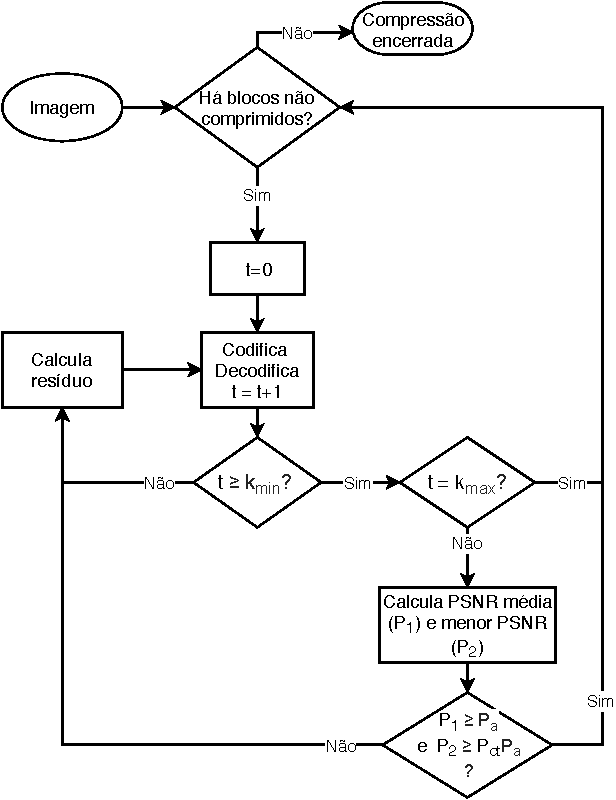
\includegraphics[width=0.7\textwidth]{figuras/fluxograma.pdf}
\caption[Método para alocação dinâmica de bit]{Método para alocação dinâmica de bits.}
\label{fig:flux_vr}
\end{figure}		

O codificador gerar um mapa de valores para indicar ao decodificador quantas iterações deve realizar por conjunto de blocos. Quando aplicamos esse métodos, lotes de tamanho 4 são utilizados com blocos $32 \times 32$. Em um lote reunimos 4096 pixels da imagem.
O número máximo de interações não ultrapassa 32 e podemos representá-lo com 5 bits. Portanto a taxa extra de bits corresponde a 0.0012 bpp. Esse valor é considerado para obter os resultados.    

\section{Implementação}

O autocodificador foi implementado usando a biblioteca PyTorch da empresa Facebook e baseado na implementação disponível em \cite{implementationRNNPytorch}. Essa biblioteca tem a vantagem de ter suporte a redes neurais construídas de forma dinâmica. Isso a torna a programação e depuração mais fácil e intuitiva em relação à biblioteca TensorFlow da Google. 
Nas demais tarefas como cálculo de métricas de qualidade e obtenção de curvas utilizamos, principalmente, a linguagem Python, e Matlab na minoria das vezes. O treinamento foi realizado em computadores com  GPU GTX 1080Ti ou GPU GTX 2080Ti. 
Em todos os testes, normalizamos os dados de entrada para o intervalo [$-0.5,0.5$] para minimizar a saturação devida as ativações sigmóides presentes no modelo. O otimizador \acrshort{adam} foi usado em todos os testes.   




